\documentclass[11pt,a4paper]{article}
\usepackage[utf8]{inputenc}\usepackage[T1]{fontenc}
\usepackage[margin=2.2cm]{geometry}
\usepackage{amsmath,amssymb,booktabs,graphicx,xcolor}
\usepackage{hyperref}\hypersetup{colorlinks=true,linkcolor=blue!55!black,urlcolor=blue!55!black}
\usepackage{caption}\captionsetup{font=small,labelfont=bf}
\usepackage{tikz}\usetikzlibrary{arrows.meta,positioning,fit,backgrounds}
\graphicspath{{figures/}}
\newcommand{\Prob}{\mathbb{P}}\newcommand{\A}[1]{\texttt{ALLOCATION\_#1}}
\title{\textbf{The blackboard game, explained from scratch}\\[2mm]
\large What the agents do, what the controller does, which pools we chose,
and how the language-model-free simulation mirrors it}
\author{MA-CC blackboard-control study}\date{4 October 2026}
\begin{document}\maketitle

\section{The task, in plain terms}

Three people must be split between two jobs: one works alone on job~1, the other
two work together on job~2. There are therefore exactly three ways to do it,
called \A{0}, \A{1} and \A{2}, one for each choice of the lone worker.

Nine hidden numbers, each 1, 2 or 3, describe the world: for each person a skill
at each job (six numbers), plus how well each pair cooperates (three numbers).
An allocation's score is
\[
\text{score} = \underbrace{\text{lone worker's skill at job 1}}_{\text{one number}}
+ \underbrace{\text{the pair's two skills at job 2}}_{\text{two numbers}}
+ \underbrace{\text{how well the pair cooperates}}_{\text{one number}} .
\]
The highest score wins. In our fixed world the hidden numbers are
$(3,1,1,2,2,1,1,1,2)$, the scores are $(8,4,6)$, so \textbf{\A{0} is correct} and
\A{2} --- the runner-up --- is the wrong answer a hostile controller tries to
promote.

\paragraph{Facts.} A \emph{fact} is a true sentence about the world, drawn from a
fixed list of 99 possible sentences (``person $p$ is at least moderately skilled
at job $j$'', ``$p$ is better than $p'$ at job $j$''). Exactly \textbf{49 of them
are true} in our world, and only those can ever be said. \textbf{Nobody ever
lies.} All the steering is done by choosing \emph{which} true things to say.

\paragraph{Belief.} Nobody sees the nine hidden numbers. But because there are
only $3^9$ possibilities, we can enumerate them: $14{,}388$ of them have a unique
winner. An agent holding a set $K$ of facts believes
\begin{equation}
\Prob(a \mid K) \;=\; \frac{\#\{\text{worlds consistent with } K \text{ where } a \text{ wins}\}}
{\#\{\text{worlds consistent with } K\}},
\label{eq:post}
\end{equation}
which is a \emph{count}, not an estimate. With no facts at all this is
$1/3$ for each allocation --- the \emph{prior}.

\section{How the full language-model simulation runs}

\begin{figure}[h]\centering
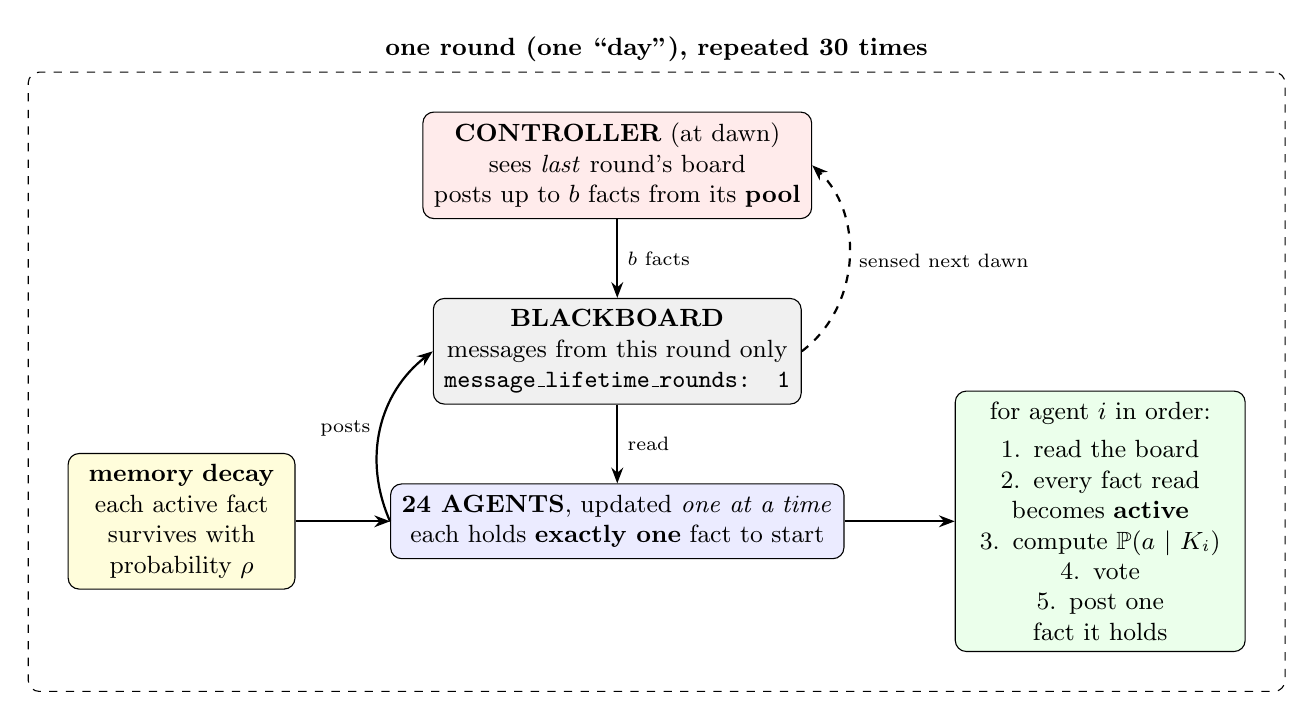
\begin{tikzpicture}[font=\small,
  box/.style={draw,rounded corners,align=center,inner sep=4pt,minimum height=8mm},
  ag/.style={box,fill=blue!8},ct/.style={box,fill=red!8},bd/.style={box,fill=black!6},
  ar/.style={-{Stealth[length=2mm]},thick}]
\node[bd,minimum width=46mm] (board) at (0,0) {\textbf{BLACKBOARD}\\ messages from this round only\\ \texttt{message\_lifetime\_rounds: 1}};
\node[ct,above=10mm of board] (ctl) {\textbf{CONTROLLER} (at dawn)\\ sees \emph{last} round's board\\ posts up to $b$ facts from its \textbf{pool}};
\node[ag,below=10mm of board] (ag) {\textbf{24 AGENTS}, updated \emph{one at a time}\\ each holds \textbf{exactly one} fact to start};
\node[box,fill=green!8,right=14mm of ag,text width=34mm] (step) {for agent $i$ in order:\\[1mm]
 1. read the board\\ 2. every fact read becomes \textbf{active}\\ 3. compute $\Prob(a\mid K_i)$\\ 4. vote\\ 5. post one fact it holds};
\node[box,fill=yellow!14,left=12mm of ag,text width=26mm] (decay) {\textbf{memory decay}\\ each active fact survives with probability $\rho$};
\draw[ar] (ctl) -- node[right,font=\scriptsize]{$b$ facts} (board);
\draw[ar] (board) -- node[right,font=\scriptsize]{read} (ag);
\draw[ar] (ag.east) -- (step.west);
\draw[ar] (decay.east) -- (ag.west);
\draw[ar] (ag.west) to[bend left=38] node[left,font=\scriptsize]{posts} (board.west);
\draw[ar,dashed] (board.east) to[bend right=50] node[right,font=\scriptsize]{sensed next dawn} (ctl.east);
\begin{scope}[on background layer]
\node[draw,dashed,rounded corners,fit=(decay)(ctl)(step),inner sep=5mm,label=above:{\textbf{one round (one ``day''), repeated 30 times}}]{};
\end{scope}
\end{tikzpicture}
\caption{One round of the game. The dashed arrow is the \emph{feedback}: the
controller's next action depends on what the population did.}
\end{figure}

\paragraph{What the agents do.} Each of the 24 agents starts holding
\textbf{exactly one} fact --- not a packet. Every round:
\begin{enumerate}\itemsep1pt
\item \textbf{Forget.} Each fact an agent currently uses survives with
probability $\rho$ (\emph{persistence}). At $\rho=1$ nothing is forgotten.
Forgotten facts are not erased, they only stop being used.
\item \textbf{Read.} The agent reads messages on the board. \textbf{Any fact it
reads becomes usable by it.} This is the only way facts spread.
\item \textbf{Think and vote.} It computes Eq.~\eqref{eq:post} from the facts it
can currently use, and votes.
\item \textbf{Post.} It writes one message citing one fact it holds.
\end{enumerate}
Agents are updated \textbf{one at a time}, so the twelfth agent sees the posts of
the first eleven. The board is wiped at the end of each round.

\paragraph{What the controller does.} It is an extra participant with its own
small set of facts --- its \textbf{pool}. Once per round, at dawn:
it looks at last round's board, decides whether to act, and if so posts up to
$b$ facts from its pool. It is given a \emph{target}: \A{0} (the truth) or
\A{2} (the wrong answer). It never lies either; it only chooses what to mention.

\paragraph{The modes that exist.}
\begin{center}\small
\begin{tabular}{llp{7.6cm}}\toprule
knob & our choice & what the alternatives mean\\\midrule
agents' communication & \texttt{report\_only} & \texttt{full\_communication} also lets agents post \emph{requests}, which carry no fact\\
board reading & \texttt{uniform}, $q{=}7$ & \texttt{full} reads every message --- but see \S4, it removes all randomness at $\rho{=}1$\\
controller action type & \texttt{adaptive\_communication} & only this and \texttt{truthful\_strategic\_report} can post a pool fact at all\\
who writes it & \texttt{llm\_authored} & \texttt{deterministic} uses a fixed rule --- and \S5 shows that rule cannot steer\\
side channel & \texttt{recommendation\_only} & \texttt{recommendation\_plus\_fact} adds one fixed fact per episode through a private channel\\
budget & $b=3$ per round & an \emph{episode} reservoir $B$ lets the controller choose \emph{when} to spend\\
gate & \texttt{always} & \texttt{soft} only fires when the population is on the wrong side of a threshold\\
\bottomrule\end{tabular}\end{center}

\section{The two setups we designed, and their pools}

Both use the \emph{same} world and the \emph{same} 49 facts. They differ only in
\textbf{which facts the 24 agents hold}.

\begin{center}\small
\begin{tabular}{lrr}\toprule
 & \textbf{symmetric-v2} & \textbf{nosolution-v2}\\\midrule
agents & 24 & 24\\
distinct facts held & 16 & 15\\
how many agents lean each way (A0/A1/A2) & 8 / 8 / 8 & 8 / 8 / 8\\
belief if you pooled every agent's facts & $(1.000,\,0,\,0)$ & $\mathbf{(0.500,\,0,\,0.500)}$\\
can the population prove the right answer? & \textbf{yes} & \textbf{no}\\
\midrule
controller pool (shared by both targets) & 12 facts & 12 facts\\
pool composition (A0/A1/A2) & 4 / 4 / 4 & 4 / 4 / 4\\
belief from the whole pool & $(\tfrac13,\tfrac13,\tfrac13)$ & $(0.318,\,0.364,\,0.318)$\\
does the pool prove anything? & \textbf{no} & \textbf{no}\\
overlap between pool and agents' facts & \textbf{0} & \textbf{0}\\
\bottomrule\end{tabular}\end{center}

\paragraph{Why one shared pool.} If the truth controller and the false
controller drew from \emph{different} pools, any difference in outcome could be
the pool rather than the policy. One pool, identical for both, means every
directional difference is attributable to \emph{what the controller chooses to
say}.

\paragraph{The plan.} Three arms --- no control, truth control, false control ---
crossed with $\rho\in\{0.75,1\}$ and the two setups: \textbf{12 cells},
100 episodes of 30 rounds each. Later, one factor at a time: the language-model
controller, full communication, the episode budget, partial sensing.

\section{The language-model-free simulation}

The same mechanism, with one substitution: wherever the real game asks a
language model to decide, we compute Eq.~\eqref{eq:post} exactly and take the
most likely allocation. No words, no tuned numbers, \textbf{no free parameters}.
A grid that would take a language model roughly 288 hours runs in
\textbf{28 seconds}.

\begin{figure}[h]\centering\includegraphics[width=\textwidth]{fig_votes_nosolution}
\caption{nosolution-v2: mean vote counts per round, in the style of the
task\_004 report. Bands are 95\% intervals. The false controller takes the
population from a near-tie to a large \A{2} majority.}
\end{figure}

\begin{figure}[h]\centering\includegraphics[width=\textwidth]{fig_votes_symmetric}
\caption{symmetric-v2: the same. In the no-control panels the population finds
the right answer on its own; the false controller takes it away even though the
agents jointly \emph{own} a proof of \A{0}.}
\end{figure}

\begin{figure}[h]\centering\includegraphics[width=0.66\textwidth]{fig_susceptibility}
\caption{Response of the three vote shares to a small change $h$ in the
controller's posting log-odds, measured as a paired finite difference at
$h=\pm0.2$, as in the task\_004 report. The three responses sum to zero by
construction. They are the same order of magnitude as the published values
($\chi_2\simeq0.019$ there).}
\end{figure}

\section{Two things the simulation taught us}

\paragraph{The repository's \texttt{deterministic} controller cannot steer.}
Its rule ranks the pool by \emph{how long ago each fact was last posted}; the
target enters only as a tie-break, and with a neutral pool it never enters at
all. Measured: the gap between the truth arm and the false arm is
\textbf{exactly zero} in all four cells, and the mutual information between the
configured target and the coarse state is \textbf{0.000 bits}, against
\textbf{1.000} for a controller that actually looks at its target.

\paragraph{Reading the whole board destroys the randomness.} At $\rho=1$ with
\texttt{sampling: full} every one of 60 episodes ends \emph{identically}. This
reverses our own earlier advice; \texttt{uniform} with $q=7$ is correct.

\section{Relation to the task\_004 thermodynamics report}

\textbf{A correction.} We previously wrote that the task\_004 paper's agent
posterior $(28/38,0,10/38)=(0.737,0,0.263)$ ``is exactly our nosolution''.
\textbf{That is wrong.} It is \texttt{task\_004} itself --- Darius's original
15-agent setup. \textbf{Our} nosolution-v2 is a redesign with a different fact
set and 24 agents, and its pooled belief is $(0.500,0,0.500)$: a coin flip, by
construction. The two are different objects and we had conflated the name
``nosolution'' with our specific redesign.

What \emph{is} exactly shared: the paper's controller pool $\mathcal F_2$, nine
facts with pooled belief $(0.0668,0,0.9332)$, is precisely the \A{2}-leaning
subset of Darius's balanced 27-fact pool. Verified.

\begin{center}\small
\begin{tabular}{p{3.4cm}p{5.2cm}p{5.2cm}}\toprule
 & \textbf{task\_004 paper} & \textbf{our simulation}\\\midrule
purpose & stochastic thermodynamics of feedback & mirror of the MA-CC runtime\\
time & continuous, Poisson thinning & discrete rounds\\
memory & \textbf{three} states: absent / passive / active & two: known / active\\
erasure & yes & \textbf{none}\\
vote & softmax on probabilities, $\beta=20$ & $\arg\max$, no parameter\\
controller pool & 9 facts, \textbf{target-specific} & 12 facts, \textbf{neutral and shared}\\
horizon / agents & 600--1000 days / 15 & 30 rounds / 24\\
free parameters & nine rates & \textbf{none}\\
\bottomrule\end{tabular}\end{center}

\paragraph{The reconciliation.} The paper's Appendix~C identifies the \emph{same}
least-recently-used ranking we did. It is not harmed by it, because \emph{its
pool is target-specific}: all nine facts favour \A{2}, so the steering lives in
the pool rather than in the ranking. Our design moves the steering into the
ranking --- and the ranking cannot carry it. Both findings are correct for their
own design.

\end{document}
